\documentclass{cys}
\usepackage[ansinew]{inputenc}

\usepackage{adjustbox}

\usepackage{graphicx}
\usepackage{tikz}
\usetikzlibrary{automata,positioning,fit}



\title{Theoretical and Experimental Approach to SMP Scheduling}

\author{Jnaneshwar Weibel}

% \affil{ 
% University of British Columbia, \authorcr
% Country             
% \authorcr \authorcr
% author1@xxx.xx
% \authorcr  \authorcr
% }

\begin{document}

\maketitle

\begin{abstract}
Over the years computer hardware has grown increasingly efficient; in particular, the capability for multiprocessing allows systems to distribute work across multiple CPUs.  Modern operating systems and their respective schedulers have the opportunity to make policy decisions about this distribution that may influence the performance of user programs.  Shared memory and locality of data ...
\end{abstract}

\begin{keywords} 
Word1, word2, word3.
\end{keywords} 

\section{Introduction}
\label{sec:introduction}
Modern computer hardware has grown increasingly efficient to improve the performance of various systems by improving areas such as processor frequency and memory latency.   While instruction throughput can be improved with optimizations to a CPU pipeline, multiprocessing is also increasingly important for improving throughput.  To improve shared memory latency, processors have adopted smaller memory subsystems, or caches, that allows quicker data access.

As the hardware evolves, software must be able to take advantage of these changes.  Within an operating system, the scheduler is responsible for running user tasks and determining an execution order; however, with multiple processors these tasks can be distributed across cores.  In a preemptive system, a task may migrate between different processors and this migration will generally impact cache performance; however, globally this migration my improve performance.  Thus several distinct policy decisions relating to task scheduling will be compared.

A run-queue will consist of a FIFO list of tasks and will be protected by a run-queue specific lock.  The performance of several tasks will be measured using a single global run-queue, a per-core run-queue without pull migration, and a per-core run-queue with pull migration.  Pull migration refers to periodically re-balancing the load on two run-queues.  In addition, some tasks will be constrained to a smaller set of CPUs and thus may be fixed to a single process or not undergo push migration.  This paper will demonstrate the performance implications that various scheduling algorithms have on both local and global task execution.

\section{Environment?}
\label{sec:environment?}
The OS will be compiled for the ARMv8 (aarch64) instruction set and will be executed on the Raspberry Pi 3 B.  The device includes a 1.2 GHz 64-bit quad-core ARM Cortex-A53 processor and consists of a 16KB L1 cache and a 128KB L2 cache.  Intra-core cache coherency is enabled and uses the MOESI protocol \cite{https://developer.arm.com/docs/ddi0500/e/level-1-memory-system/cache-behavior/data-cache-coherency}.  The memory address space is configured using a linear two level translation table with accessible memory configured as normal outer and inner write-back, write-allocate and device register memory configured as device nGnRnE.  Performance will be measured using the ARM Performance Monitor Unit (PMU) and the core timer.  The timer executes at a frequency of 19.2 MHz and each core maintains its own core timer which will preempt the current task each MS. \cite{https://www.raspberrypi.org/documentation/hardware/raspberrypi/bcm2836/QA7_rev3.4.pdf}

\section{Definitions}
\label{sec:definitions}

A ready queue can be defined as a generic data structure with two primary operations: ready and next.  For its internal manipulation a ready queue is protected by a spinlock.  Internally there are several queues corresponding to different priority levels allowing for processes with different priorities to be pushed onto the queues with no contention.  However, for discussion we will assume that all processes run at the same priority.

A naieve implementation for a SMP scheduler involves a global ready queue which all cores pull processes from.  This naieve implementation acts identical that in a single core system.  On SMP systems this data structure is benificial since it guarantees equal distribution of workload across all cores in addition to implementation simplicity.  Additionally, this workload distribution is not affected by a rapid stream of exiting processes. (TODO possibly example)  However, the approach suffers from kernel lock contention since all cores must synchronize access to the queue.

\begin{figure}
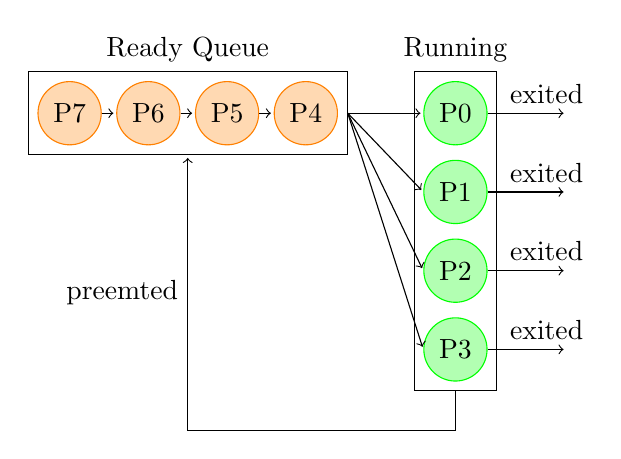
\begin{tikzpicture}[shorten >=1pt,node distance=1.0cm,on grid,auto,
    running/.style={circle, draw=green!100, fill=green!30},
    ready/.style={circle, draw=orange!100, fill=orange!30}
    ]

    \node[ready] (p_4) [] {P4};
    \node[ready] (p_5) [left=of p_4] {P5};
    \node[ready] (p_6) [left=of p_5] {P6};
    \node[ready] (p_7) [left=of p_6] {P7};

    \node[state,rectangle] (q_0) [fit={(p_4) (p_5) (p_6) (p_7)}] [label=Ready Queue] {};

    \node[running] (r_0) [right=of q_0, xshift=24mm] {P0};
    \node[running] (r_1) [below=of r_0] {P1};
    \node[running] (r_2) [below=of r_1] {P2};
    \node[running] (r_3) [below=of r_2] {P3};

    \node[state,rectangle] (q_1) [fit={(r_0) (r_1) (r_2) (r_3)}] [label=Running] {};

    \draw[->] (q_0.east) -- (r_0.west);
    \draw[->] (q_0.east) -- (r_1.west);
    \draw[->] (q_0.east) -- (r_2.west);
    \draw[->] (q_0.east) -- (r_3.west);

    \draw[->] (p_7.east) -- (p_6.west);
    \draw[->] (p_6.east) -- (p_5.west);
    \draw[->] (p_5.east) -- (p_4.west);

    \draw[->] (r_0.east) -- ++(10mm,0) node[near end] {exited};
    \draw[->] (r_1.east) -- ++(10mm,0) node[near end] {exited};
    \draw[->] (r_2.east) -- ++(10mm,0) node[near end] {exited};
    \draw[->] (r_3.east) -- ++(10mm,0) node[near end] {exited};
     
    \draw[->] (q_1.south) |- ++(0,-5mm) -| (q_0.south) node[near end] {preemted};
\end{tikzpicture}
\caption{Global Ready Queue}
\end{figure}

\begin{figure}
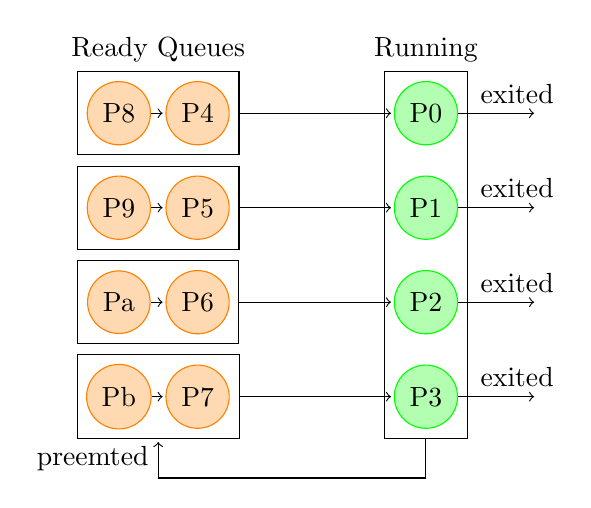
\begin{tikzpicture}[shorten >=1pt,node distance=1.0cm,on grid,auto,
    running/.style={circle, draw=green!100, fill=green!30},
    ready/.style={circle, draw=orange!100, fill=orange!30}
    ]

    \node[ready] (p_4) [] {P4};
    \node[ready] (p_5) [below=of p_4, yshift=-2mm] {P5};
    \node[ready] (p_6) [below=of p_5, yshift=-2mm] {P6};
    \node[ready] (p_7) [below=of p_6, yshift=-2mm] {P7};

    \node[ready] (p_8) [left=of p_4] {P8};
    \node[ready] (p_9) [left=of p_5] {P9};
    \node[ready] (p_10) [left=of p_6] {Pa};
    \node[ready] (p_11) [left=of p_7] {Pb};    

    \node[state,rectangle] (q_0) [fit={(p_4) (p_8)}] [label=Ready Queues] {};
    \node[state,rectangle] (q_1) [fit={(p_5) (p_9)}] [below=of q_0, yshift=-2mm] {};
    \node[state,rectangle] (q_2) [fit={(p_6) (p_10)}] [below=of q_1, yshift=-2mm] {};
    \node[state,rectangle] (q_3) [fit={(p_7) (p_11)}] [below=of q_2, yshift=-2mm] {};

    \node[running] (r_0) [right=of q_0, xshift=24mm] {P0};
    \node[running] (r_1) [below=of r_0, yshift=-2mm] {P1};
    \node[running] (r_2) [below=of r_1, yshift=-2mm] {P2};
    \node[running] (r_3) [below=of r_2, yshift=-2mm] {P3};

    \node[state,rectangle] (q_r) [fit={(r_0) (r_1) (r_2) (r_3)}] [label=Running] {};

    \draw[->] (q_0.east) -- (r_0.west);
    \draw[->] (q_1.east) -- (r_1.west);
    \draw[->] (q_2.east) -- (r_2.west);
    \draw[->] (q_3.east) -- (r_3.west);

    \draw[->] (p_8.east) -- (p_4.west);
    \draw[->] (p_9.east) -- (p_5.west);
    \draw[->] (p_10.east) -- (p_6.west);
    \draw[->] (p_11.east) -- (p_7.west);
     
    \draw[->] (q_r.south) |- ++(0,-5mm) -| (q_3.south) node[near end] {preemted};
    \draw[->] (r_0.east) -- ++(10mm,0) node[near end] {exited};
    \draw[->] (r_1.east) -- ++(10mm,0) node[near end] {exited};
    \draw[->] (r_2.east) -- ++(10mm,0) node[near end] {exited};
    \draw[->] (r_3.east) -- ++(10mm,0) node[near end] {exited};
\end{tikzpicture}
\caption{Per Core Ready Queue}
\end{figure}

Under the current scheduler, a process, if eligible, is migrated during preemption.  In general the scheduler will opt to keep a process on the same CPU unless another core is sufficiently empty or its affinity set dictates otherwise.  In essence this rebalancing means that as processes are rescheduled, the cores will tend towards a balanced configuration.  However, it is also possible that a core will have a stream of processes terminate leading to a load imbalance between ready queues (fig. 3).

\begin{figure}
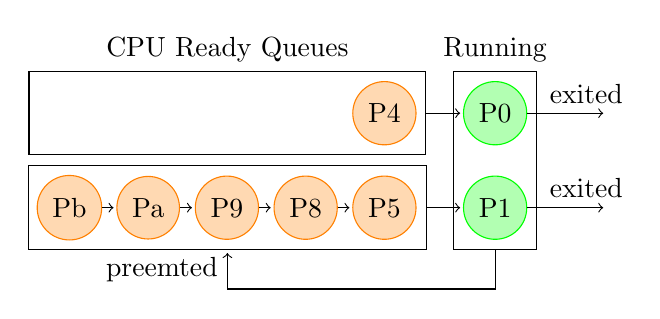
\begin{tikzpicture}[shorten >=1pt,node distance=1.0cm,on grid,auto,
    running/.style={circle, draw=green!100, fill=green!30},
    ready/.style={circle, draw=orange!100, fill=orange!30},
    empty/.style={circle, draw=none, fill=none, text=white}
    ]

    \node[ready] (p_4) [] {P4};
    \node[ready] (p_5) [below=of p_4, yshift=-2mm] {P5};

    \node[ready] (p_6) [left=of p_5] {P8};
    \node[ready] (p_7) [left=of p_6] {P9};
    \node[ready] (p_8) [left=of p_7] {Pa};
    \node[ready] (p_9) [left=of p_8] {Pb}; 
    
    \node[empty] (p_e) [above=of p_9, yshift=+2mm] {Pe};

    \node[state,rectangle] (q_0) [fit={(p_4) (p_e)}] [label=CPU Ready Queues] {};
    \node[state,rectangle] (q_1) [fit={(p_5) (p_6) (p_7) (p_8) (p_9)}] [below=of q_0, yshift=-2mm] {};

    \node[running] (r_0) [right=of q_0, xshift=24mm] {P0};
    \node[running] (r_1) [below=of r_0, yshift=-2mm] {P1};

    \node[state,rectangle] (q_r) [fit={(r_0) (r_1)}] [label=Running] {};

    \draw[->] (q_0.east) -- (r_0.west);
    \draw[->] (q_1.east) -- (r_1.west);

    \draw[->] (p_9.east) -- (p_8.west);
    \draw[->] (p_8.east) -- (p_7.west);
    \draw[->] (p_7.east) -- (p_6.west);
    \draw[->] (p_6.east) -- (p_5.west);
     
    \draw[->] (q_r.south) |- ++(0,-5mm) -| (q_1.south) node[near end] {preemted};
    \draw[->] (r_0.east) -- ++(10mm,0) node[near end] {exited};
    \draw[->] (r_1.east) -- ++(10mm,0) node[near end] {exited};
\end{tikzpicture}
\caption{Unbalanced Scheduling}
\end{figure}

Pull migration is an effort to improve the rebalancing latency for queues which exhibit the behaivour in fig. 3.  Periodically, an idle core will search for an overloaded core and pull eligible processes from the tail of its queue.  This task requires locking the busy queue for a longer period of time; while, the idle queue tends to have have its lock acquired more frequently.  This task leads to high lock contention for both queues which can negatively impact the time spent in the kernel.  Specifically, while iterating, the busy core will be unable to retrieve the next runnable process.  Thus it is important to pick a large enough interval to do the rebalancing that it does not cause much strain on performance.  However, in most cases, if a core is not sufficiently loaded the pull migration task will instead exit prematurely instead of locking both cores.


\section{Performance Tests}
\label{sec:perfTests}
Various user programs were tested against different variations of the scheduler.  In general the tests were performed on processes tasked with performing a scalar multiply on a data set with a size relative to the L1 cache.  As a baseline, the OS was configured to run on only a single core and a matrix multiplication was performed on a matrix exactly the size of the cache.  For more interesting results, a data set 4x the size of the cache was tested with the global run-queue and the per-core run-queue with evenly distributed CPU affinity.  In these cases each process would work on an independent part of the data set.  

The impact of per-core scheduler with and without pull migration was analyzed with tasks with varying runtime.  Three classes of processes were defined as short, medium and long; each, with 10x the runtime of the previous case.  An even distribution of each type of task and the data set was tested against these schedulers.  Additionally the schedulers were tested against many short runtime processes compared to the few long runtime processes.

Finally, a common pattern; in resource intensive and parallelizable tasks, is to create a smaller subset of OS tasks and pull work off a shared queue.  Otherwise known as a thread pool, the difference between allowing the OS to manage all the tasks compared to semi-manual work queueing was examined.  Work was divided into 64 threads with 16 workers for the pooled case.  Additionally the locality of the data being worked on was constrained to both 4 (sm) and 16 (lg) matrices of a smaller size than the L1 cache.  All tests ran on the per-core scheduler with pull migration.  

% \begin{table}[h!]
%     \centering
%     \caption{Table to test captions and labels}
% \end{table}

In general for the following examples the runtime gives a rough measurement of elapsed jiffies.  However, the cycle count provides a better perforamnce measurement.  Additionally, it is important to all data is cached in the L2 cache and thus stalls for fetching from main memory are generally minimized.

\begin{table}[h!]
    \centering
    \adjustbox{max width=\columnwidth}{\begin{tabular}{ l|rrr }
        Type & Total & User & Kernel \\
        \hline
        Instrs & 467617788 & 466380022 & 1237766 \\ 
        Cycles & 693267321 & 691411106 & 1856215 \\ 
        Access & 264291472 & 263665636 & 625836 \\ 
        Refill & 1539 & 1340 & 199 \\ 
        Runtime & 45374884 & - & - \\ 
        \hline
    \end{tabular}}
    \caption{single core - matrix 1x utilization}
\end{table}

\begin{table}[h!]
    \centering
    \adjustbox{max width=\columnwidth}{\begin{tabular}{ l|rrr }
        Type & Total & User & Kernel \\
        \hline
        Instrs & 1858506765 & 1853566311 & 4940454 \\ 
        Cycles & 2768987855 & 2760678046 & 8309809 \\ 
        Access & 1050488228 & 1047990323 & 2497905 \\ 
        Refill & 1389770 & 1293188 & 96582 \\ 
        Runtime & 178608294 & - & - \\ 
        \hline
    \end{tabular}}
    \caption{single core - matrix 4x utilization}
\end{table}

This initial example aims to show the stark difference between process cache utilization.  The two examples operate on a matrix fully utilizes the L1 cache and overloads the cache in the second instance.  It is important to note that while the cycle count is nearly 4x larger as expected, the refill rate for the larger matrix is larger by a factor of nearly 900x.  In these examples the most noticeable difference is the instructions per cycle in the kernel being roughly 11\% slower, due to the frequent thrashing of kernel memory. 

\begin{table}[h!]
    \centering
    \adjustbox{max width=\columnwidth}{\begin{tabular}{ l|rrr }
        Type & Total & User & Kernel \\
        \hline
        Instrs & 354249559 & 353629318 & 620241 \\ 
        Cycles & 527538552 & 526403550 & 1135002 \\ 
        Access & 200305644 & 199963039 & 342605 \\ 
        Refill & 125708 & 116722 & 8986 \\ 
        Runtime & 41175374 & - & - \\ 
        \hline
    \end{tabular}}
    \caption{multi core - global queue}
\end{table}

\begin{table}[h!]
    \centering
    \adjustbox{max width=\columnwidth}{\begin{tabular}{ l|rrr }
        Type & Total & User & Kernel \\
        \hline
        Instrs & 375176881 & 374755150 & 421731 \\ 
        Cycles & 556693572 & 556049701 & 643871 \\ 
        Access & 212114934 & 211903384 & 211550 \\ 
        Refill & 15332 & 14735 & 597 \\ 
        Runtime & 40603738 & - & - \\ 
        \hline
    \end{tabular}}
    \caption{multi core - cpu queue (affinity)}
\end{table}

Extending the trivial example to multicore serves as a demonstration of easily parallelizable code and the benefit of process affinity.  For this example, the instructions per cycle is nearly 1\% faster in the kernel for the case with constrained affinity.  Again, the kernel data structures generally remain in the L1 cache as evident by the a lower number of access per refill \approx 1.6\% in the global runqueue case.  It is also important to note that the number of kernel instructions is \approx 68\% less in the per core runqueue, howing to less lock contention between cores.

\begin{table}[h!]
    \centering
    \adjustbox{max width=\columnwidth}{\begin{tabular}{ l|rrr }
        Type & Total & User & Kernel \\
        \hline
        Instrs & 1543135939 & 1396850683 & 146285256 \\ 
        Cycles & 3146576481 & 2076522276 & 1070054205 \\ 
        Access & 845516444 & 789349384 & 56167060 \\ 
        Refill & 7653514 & 112360 & 7541154 \\ 
        Runtime & 152657484 & - & - \\
        \hline
    \end{tabular}}
    \caption{death - no pull sm}
\end{table}

\begin{table}[h!]
    \centering
    \adjustbox{max width=\columnwidth}{\begin{tabular}{ l|rrr }
        Type & Total & User & Kernel \\
        \hline
        Instrs & 1468299596 & 1398454567 & 69845029 \\ 
        Cycles & 2552848279 & 2079318879 & 473529400 \\ 
        Access & 816022596 & 790256656 & 25765940 \\ 
        Refill & 3126952 & 140213 & 2986739 \\ 
        Runtime & 156804356 & - & - \\ 
        \hline
    \end{tabular}}
    \caption{death - pulled sm}
\end{table}

\begin{table}[h!]
    \centering
    \adjustbox{max width=\columnwidth}{\begin{tabular}{ l|rrr }
        Type & Total & User & Kernel \\
        \hline
        Instrs & 1613944771 & 1404552990 & 209391781 \\ 
        Cycles & 3491698429 & 2086636583 & 1405061846 \\ 
        Access & 873214573 & 793699999 & 79514574 \\ 
        Refill & 9792188 & 28820 & 9763368 \\ 
        Runtime & 152321428 & - & - \\ 
        \hline
    \end{tabular}}
    \caption{death - no-pull}
\end{table}

The previous examples operate on _______.  TODO: this case needs fleshing out...
specific pattern likely samples of the same matrix get flushed to the idle cores.  May want to repeat these tests with affinity for the idle procs.

\begin{table}[h!]
    \centering
    \adjustbox{max width=\columnwidth}{\begin{tabular}{ l|rrr }
        Type & Total & User & Kernel \\
        \hline
        Instrs & 1520575475 & 1445743126 & 74832349 \\ 
        Cycles & 2574353547 & 2147872630 & 426480917 \\ 
        Access & 843643737 & 816978128 & 26665609 \\ 
        Refill & 2283806 & 34930 & 2248876 \\ 
        Runtime & 161631896 & - & - \\ 
        \hline
    \end{tabular}}
    \caption{death - pulled}
\end{table}

\begin{table}[h!]
    \centering
    \adjustbox{max width=\columnwidth}{\begin{tabular}{ l|rrr }
        Type & Total & User & Kernel \\
        \hline
        Instrs & 2945961318 & 2829092653 & 116868665 \\ 
        Cycles & 4881259967 & 4206238780 & 675021187 \\ 
        Access & 1642115209 & 1598721424 & 43393785 \\ 
        Refill & 4570467 & 298213 & 4272254 \\ 
        Runtime & 175864992 & - & - \\
        \hline
    \end{tabular}}
    \caption{runtime - no pull}
\end{table}

% \begin{table}[h!]
%     \centering
%     \adjustbox{max width=\columnwidth}{\begin{tabular}{ l|rrr }
%         Type & Total & User & Kernel \\
%         \hline
%         Instrs & 2727027846 & 2625810066 & 101217780 \\ 
%         Cycles & 4421745433 & 3903078399 & 518667034 \\ 
%         Access & 1520521397 & 1483845439 & 36675958 \\ 
%         Refill & 3226996 & 222090 & 3004906 \\ 
%         Runtime & 171909144 & - & - \\
%         \hline
%     \end{tabular}}
%     \caption{runtime - pulled}
% \end{table}

% \begin{table}[h!]
%     \centering
%     \adjustbox{max width=\columnwidth}{\begin{tabular}{ l|rrr }
%         Type & Total & User & Kernel \\
%         \hline
%         Instrs & 836416320 & 753346040 & 83070280 \\ 
%         Cycles & 1724034904 & 1123196400 & 600838504 \\ 
%         Access & 456170314 & 426134109 & 30036205 \\ 
%         Refill & 4027452 & 231590 & 3795862 \\ 
%         Runtime & 165276806 & - & - \\
%         \hline
%     \end{tabular}}
%     \caption{pool - unpooled sm}
% \end{table}

% \begin{table}[h!]
%     \centering
%     \adjustbox{max width=\columnwidth}{\begin{tabular}{ l|rrr }
%         Type & Total & User & Kernel \\
%         \hline
%         Instrs & 811243405 & 741653152 & 69590253 \\ 
%         Cycles & 1789217832 & 1113471653 & 675746179 \\ 
%         Access & 444450115 & 419398612 & 25051503 \\ 
%         Refill & 4540858 & 379326 & 4161532 \\ 
%         Runtime & 66534692 & - & - \\
%         \hline
%     \end{tabular}}
%     \caption{pool - pooled sm}
% \end{table}

\begin{table}[h!]
    \centering
    \adjustbox{max width=\columnwidth}{\begin{tabular}{ l|rrr }
        Type & Total & User & Kernel \\
        \hline
        Instrs & 819345284 & 755845609 & 63499675 \\ 
        Cycles & 1672284752 & 1125235476 & 547049276 \\ 
        Access & 450878090 & 427546852 & 23331238 \\ 
        Refill & 3740754 & 148469 & 3592285 \\ 
        Runtime & 167143162 & - & - \\ 
        \hline
    \end{tabular}}
    \caption{pool - unpooled}
\end{table}

\begin{table}[h!]
    \centering
    \adjustbox{max width=\columnwidth}{\begin{tabular}{ l|rrr }
        Type & Total & User & Kernel \\
        \hline
        Instrs & 840132648 & 753613514 & 86519134 \\ 
        Cycles & 1849770029 & 1127098953 & 722671076 \\ 
        Access & 457128942 & 426166739 & 30962203 \\ 
        Refill & 4435166 & 143616 & 4291550 \\ 
        Runtime & 66158114 & - & - \\ 
        \hline
    \end{tabular}}
    \caption{pool - pooled}
\end{table}


\subsection{Linguistic Features}
\label{subsection:linguistic}

Features. 

\subsubsection{Lexical Features}
\label{subsection:lexicalFeatures}

Other features.

\begin{equation}
H(X|Y) = - \sum_{y \in Y} P(y_i) \sum_{x \in X} p(x_i|y_i)\log p(x_i|y_i)
\label{equation:conditionalEntropy1}
\end{equation}


\section{Conclusion and Future Work}
\label{sec:conclusionAndFutureWork}

Conclusions here.

\section{Acknowledgements} 
We would like to thank.. 



% OBLIGATORY: use BIBTEX formatting!
\small{
\bibliographystyle{cys}
\bibliography{biblio}
}
\normalsize

\end{document}

